\documentclass[11pt]{article}
\usepackage[margin=1in]{geometry}
\usepackage{amsmath,amssymb}
\usepackage{booktabs}
\usepackage{array}
\usepackage{enumitem}
\usepackage[hidelinks]{hyperref}
\usepackage{xurl}
\usepackage{threeparttable}
\usepackage{graphicx}
\setlist{nosep}

\newcommand{\bn}{\$bn}

\title{Sizing the US stock of data-center facilities:\\ four sources, one object}
\author{}
\date{September 2026. Working note, P\&P project.}

\begin{document}
\maketitle

\begin{abstract}
\noindent We estimate the US net stock of hyperscale and colocation data-center facilities, defined as the building plus the installed power and cooling plant and excluding servers, from four independent sources: Census construction spending cumulated by the perpetual-inventory method, BEA fixed assets by owner industry, company filings, and physical capacity in megawatts times construction cost per megawatt. We first document where data centers sit in the official system: NAICS classifies a captive data center by its own activity, BEA fixed assets are on an establishment basis fed by a company-level survey, and the Census construction category includes mechanical and electrical plant but not racks. For 2018 the construction cumulation gives \$33bn, filings \$44--69bn, the inventory route \$26--44bn, and the owner-industry total \$84bn before deducting offices; the ranges overlap at \$45--70bn. For 2024 the same sources give \$143bn, \$179--269bn, \$158--248bn and \$304bn. The owner-industry total reconciles with filings only if all four large cloud providers and the colocation operators report their data centers in the hosting industry. The main lessons for calibration are that the construction series understates the level before 2020, that a construction-based stock already contains the power and cooling plant and should not be topped up with a separate equipment stock, and that the type split inside BEA's fixed assets is not stable across vintages and should not be used as an anchor.
\end{abstract}

\section{Objective}

A data center is two things in the national accounts. It is a capital good, a building with electrical and cooling plant that houses servers, and it is a producing establishment that sells computing and hosting services. This note is about the first object, and about one number: the dollar value of the US stock of data-center facilities at a date, net of depreciation, excluding the IT equipment inside.

We need this number to size a data-center facilities sector in a multi-sector production and investment network. Its capital stock times a rental rate is the sector's capital income; its depreciation times the stock is its steady-state investment; the composition of that investment is a column of the investment network. Every downstream cell scales with it.

No official series measures it directly. We therefore triangulate from four sources that see the object from different angles: what was built (construction spending), what owners hold (fixed assets by industry), what listed companies report (10-K filings), and what physically exists (megawatts of installed capacity). Section~\ref{sec:where} sets out where data centers sit in the official system, because the interpretation of two of the four sources depends on it. Section~\ref{sec:angles} works through each source with its data, method and caveats. Section~\ref{sec:reconcile} puts them side by side.

\section{The object}

Throughout, ``facility'' means the shell and site works plus the installed mechanical and electrical plant: transformers, switchgear, uninterruptible power supplies, generators, chillers, cooling distribution. It excludes land, racks, servers, storage and networking gear. The split matters for two reasons. First, the plant is most of the cost: in the 2025 Turner \& Townsend cost index for US air-cooled builds, shell and architectural work is 14\% of construction cost, mechanical 22\%, electrical 54\%, and general conditions 10\%. A ``structures'' number for a data center is mostly power and cooling plant. Second, the plant depreciates at roughly 10\% a year while the shell depreciates at 2--3\%, so a construction-based stock has a blended rate near 8--9\%, not the 2.5\% BEA applies to office buildings.

We focus on hyperscale and colocation facilities, that is, purpose-built capacity operated by cloud providers or leased to them and to enterprises. Enterprise server rooms inside office buildings, government facilities and crypto mines are excluded where the source allows and flagged where it does not.

Stocks are net of depreciation at current cost unless stated. Where a source gives gross replacement cost we convert with an assumed age profile, stated in the relevant subsection.

\section{Where data centers sit in the official system}
\label{sec:where}

\paragraph{Industry classification.} NAICS classifies establishments by their own activity, including establishments that exist only to serve other units of the same enterprise. The 2022 manual states that units carrying out support activities for their enterprise are classified ``according to the NAICS code related to their own activity,'' with the example that a warehouse storing its own enterprise's goods is a warehouse. A Google or Amazon data center serving only Google or Amazon is therefore a data-processing and hosting establishment, NAICS 518210, and not a search portal or a retailer. The 2022 revision of 518210 (``Computing Infrastructure Providers, Data Processing, Web Hosting, and Related Services'') lists infrastructure-as-a-service, platform-as-a-service and colocation among its activities. In BEA's 71-industry accounts, 518 is combined with 519 into industry 514, ``Data processing, internet publishing, and other information services,'' which also contains web search portals (Google) and internet publishing (Meta).

\paragraph{Fixed assets by industry.} BEA's fixed-asset accounts assign assets to the industry of the establishment that uses them. The stated basis is the establishment, and the methodology notes that ``assets are classified in the industry that purchases them.'' The main source for investment by industry since 2002, however, is the Census Annual Capital Expenditures Survey (ACES), which samples companies. ACES asks multi-industry companies to split capital expenditures by industry (item 6A), so the published statistics are, in BEA's words, ``closer to an establishment basis.'' BEA's own working paper on the topic notes that a non-manufacturing establishment of a manufacturing company can be reported under manufacturing in ACES even though the Economic Census would put it under non-manufacturing. Whether a hyperscaler's data centers are reported under 514 or under the parent's main line (software publishing for Microsoft, retail for Amazon) depends on how the company fills in item 6A. Within an industry, the allocation of structures investment to building types (office, communication, manufacturing, and so on) comes from asset-type detail collected in the ACES in the year after each Economic Census, balanced to Census construction-spending totals by type. Since 2010 BEA presents structure types by function, following the Census classification of construction put in place.

\paragraph{Construction spending.} The Census Value of Construction Put in Place (C30) added a ``Data center'' line under private office construction in the May 2024 release, monthly back to January 2014. The definition is ``buildings that contain the hardware needed for storing, processing, and transmitting digital information.'' Construction cost includes ``mechanical and electrical installations such as plumbing, heating, electrical work, elevators, escalators, central air-conditioning, emergency backup power,'' and excludes ``special purpose equipment \ldots\ such as \ldots\ racks or servers in data centers.'' Projects are drawn from the Dodge project frame with the owner as respondent, so owner-built campuses are in scope if Dodge lists them; BEA notes that the survey ``may or may not fully capture'' own-account projects. Since the September 2025 annual update, NIPA table 5.4.5U carries a ``Data centers'' line under office structures sourced from this series.

\paragraph{Depreciation.} BEA's geometric rates are 0.0247 for office buildings (36-year life), 0.0237 for communication structures (40 years) and 0.0314 for manufacturing structures (31 years). Computers and peripherals have no geometric rate; BEA uses empirical used-price profiles that imply 35--45\% a year after the first year. The implied structures rate for industry 514 in the detailed accounts is 0.025--0.030.

\paragraph{Consequences for measurement.} Three follow. A hyperscaler's data centers should appear in industry 514 fixed assets, but in practice may not, depending on company reporting; the same industry also holds Google's and Meta's office campuses, so 514 structures are an upper bound for data centers. Colocation REITs are 518210 by activity but may be booked to real estate as lessors; there is no way to recover them from the real-estate industry's \$1.4 trillion of structures. And a stock built from C30 already contains the power and cooling plant, so adding a separate equipment stock for that plant double counts.

\section{Four angles}
\label{sec:angles}

\subsection{Construction spending cumulated}
\label{sec:c30}

\paragraph{Data.} Annual totals of the C30 data-center line, seasonally adjusted, in \bn: 1.8 (2014), 2.7, 4.1, 4.7, 6.9 (2018), 8.5, 9.2, 9.9, 12.6 (2022), 20.0, 34.7 (2024), 49.7 (2025).

\paragraph{Method.} Perpetual inventory, $K_t=(1-\delta)K_{t-1}+I_t$, in constant dollars, revalued to current cost each year. The deflator is the NIPA price index for office structures investment (table 5.4.4, line 4; 2025 extended with the commercial and health care index). The series starts in 2014, so the end-2013 stock must be assumed; we set $K_{2013}=I_{2014}/(\delta+g)$ with a pre-sample growth rate $g$. We show two depreciation rates: 0.03, close to BEA's rate for the building types involved, and 0.085, a blend of 0.03 on the 15\% shell share and 0.10 on the 85\% plant share.

\paragraph{Result.} With $\delta=0.03$ and $g=0.10$ the current-cost stock is \$33bn at end-2018, \$87bn at end-2022, \$143bn at end-2024 and \$191bn at end-2025. With $\delta=0.085$ it is \$26bn, \$67bn, \$115bn and \$156bn. The pre-sample anchor accounts for about a third of the 2018 stock and under a tenth of the 2024 stock. Table~\ref{tab:pim} shows the sensitivity.

\begin{table}[ht]
\centering
\begin{threeparttable}
\caption{Current-cost stock from C30 cumulation, \bn}
\label{tab:pim}
\begin{tabular}{llccccc}
\toprule
$\delta$ & Year & $g=0.05$ & $g=0.10$ & $g=0.20$ & $g=0.40$ & $K_{2013}=0$ \\
\midrule
0.03  & 2018 & 41.6 & 33.3 & 27.6 & 24.2 & 20.2 \\
      & 2022 & 96.6 & 86.5 & 79.5 & 75.3 & 70.5 \\
      & 2024 & 153.8 & 143.4 & 136.2 & 131.9 & 126.8 \\
0.085 & 2018 & 28.1 & 25.6 & 23.2 & 21.3 & 18.7 \\
      & 2022 & 69.4 & 67.0 & 64.6 & 62.8 & 60.3 \\
      & 2024 & 116.8 & 114.5 & 112.4 & 110.7 & 108.4 \\
\bottomrule
\end{tabular}
\begin{tablenotes}\footnotesize
\item $K_{2013}=I_{2014}/(\delta+g)$. Accumulated in 2017 dollars and revalued with the office structures price index. Undeflated accumulation gives \$31bn, \$66bn and \$117bn for $\delta=0.03$, $g=0.10$.
\end{tablenotes}
\end{threeparttable}
\end{table}

\paragraph{Caveats.} The series undercounts if hyperscale campuses were reported under office, warehouse or industrial categories before the line existed, or if own-account projects are missing from the Dodge frame. Industry 514 structures investment ran 2--4 times the C30 line in every year 2014--2022 (Section~\ref{sec:fa}), which is consistent with undercounting. On the other side, C30 counts contractor cost including installed plant, so the stock it produces is a facility stock, not a shell stock; this is the right object for us but should not be read as ``structures'' in the BEA sense.

\subsection{BEA fixed assets by owner industry}
\label{sec:fa}

\paragraph{Data.} Current-cost net stocks of nonresidential structures by type, from the detailed fixed-asset tables for industry 514 (BEA sheet code 5140), September 2025 release. Table~\ref{tab:fa} reports the totals, the building types that carry the growth, and the server stock of the same establishments.

\begin{table}[ht]
\centering
\begin{threeparttable}
\caption{Industry 514 net stock, current cost, \bn}
\label{tab:fa}
\small
\begin{tabular}{lrrrrrrrr}
\toprule
 & 2005 & 2010 & 2014 & 2016 & 2018 & 2020 & 2022 & 2024 \\
\midrule
Total structures & 10.0 & 19.4 & 34.3 & 55.4 & 84.0 & 133.1 & 235.2 & 304.4 \\
\quad Office & 7.6 & 11.5 & 18.0 & 28.1 & 43.1 & 71.3 & 135.2 & 171.4 \\
\quad Communication & 0.4 & 3.7 & 9.3 & 17.7 & 28.9 & 46.4 & 75.7 & 103.8 \\
\quad Manufacturing & 0.1 & 1.4 & 3.8 & 6.2 & 6.4 & 6.5 & 8.6 & 8.6 \\
\quad Electric & 0.0 & 0.0 & 0.0 & 0.0 & 1.6 & 4.0 & 7.9 & 10.9 \\
\quad Other & 1.9 & 2.8 & 3.1 & 3.3 & 4.1 & 5.0 & 7.9 & 9.7 \\
\midrule
Structures investment & -- & 3.5 & 7.5 & 12.0 & 17.6 & 26.2 & 33.3 & 36.9 \\
\midrule
Servers & 2.1 & 6.8 & 16.9 & 20.7 & 29.1 & 33.8 & 51.6 & 65.0 \\
Total equipment & 17.3 & 28.2 & 53.6 & 70.3 & 106.1 & 129.8 & 193.6 & 245.5 \\
\bottomrule
\end{tabular}
\begin{tablenotes}\footnotesize
\item ``Servers'' is asset codes EP1A (mainframes), EP1G (storage), EP1H (system integrators). BEA flags industry-by-asset detail cells as lower quality than the aggregates. In the August 2019 release the 2018 column read 85.9 total, 38.1 office, 25.3 communication and 19.3 manufacturing.
\end{tablenotes}
\end{threeparttable}
\end{table}

\paragraph{Method.} The industry total is an owner-based measure of everything industry 514 establishments hold. To read it as a data-center stock one must subtract genuine offices and add data centers held elsewhere.

\paragraph{Result.} Total structures grew from \$10bn in 2005 to \$84bn in 2018, \$235bn in 2022 and \$304bn in 2024. Structures investment by the industry was 2--4 times the C30 data-center line in every year 2014--2022; in 2024 the two are equal (\$36.9bn against \$34.7bn). The type split is not stable across vintages. For 2018 the 2025 release moved \$13bn out of ``manufacturing'' and into ``office'' and ``communication'' relative to the 2019 release, with the total almost unchanged. In the 2019 vintage the growth of communication and manufacturing buildings inside a services industry looked like the footprint of data centers; in the 2025 vintage most of that footprint is under office, presumably because BEA now follows the Census placement of data centers under office construction. Office is 56\% of the total in both 2018 and 2024.

\paragraph{Caveats.} The industry includes Google and Meta, whose office campuses are large; the office deduction is estimated from their disclosed square footage in Section~\ref{sec:filings}. Microsoft's facilities may sit in software publishing (industry 511), whose structures grew from \$44bn in 2010 to \$60bn in 2018 and \$92bn in 2024 with no visible break; Amazon's may sit in retail, whose communication-type structures are near zero, which suggests AWS is reported under 514. Colocation REITs may be in real estate, whose communication-type structures are flat at \$2bn, and are then unrecoverable. The detail cells are flagged low quality by BEA. Net: the industry total is a firm upper bound on hyperscale-plus-colocation facilities held by 514 establishments, and the type split should not be used.

\subsection{Company filings}
\label{sec:filings}

\paragraph{Data.} Balance-sheet property, plant and equipment from 10-K filings (SEC XBRL company facts and the PP\&E and Properties notes), fiscal 2018, 2022 and 2024. Colocation REITs: Equinix, Digital Realty, CyrusOne, QTS, CoreSite, and Iron Mountain's data-center segment; from 2022 also American Tower's data-center segment (CoreSite). Hyperscalers: Alphabet, Microsoft, Amazon, Meta, Oracle. For the leased capacity that filings do not see after 2021, we add megawatts from Section~\ref{sec:mw} priced at construction cost.

\paragraph{Method.} For REITs, net ``buildings and improvements'' (which capitalise the installed plant) less land and personal property, times the US share of revenue from the geographic note. For hyperscalers, gross ``buildings'' from the PP\&E note, times a net-to-gross factor of 0.70--0.82 (no company discloses accumulated depreciation by asset class), times a data-center share of buildings, times the US share of property. The data-center share is the weakest input and Appendix~\ref{app:hyp} lists the disclosure behind each range. The one hard number is Alphabet's 2025 statement that about 60\% of its technical infrastructure is servers and network equipment and the rest data-center land and buildings, which puts Alphabet's data-center buildings at about \$56bn gross in 2024, and the data-center share of Alphabet's buildings (offices \$44bn) at 56\%. Amazon reports AWS segment property of \$18.9bn, \$60.3bn and \$110.7bn net in the three years, and AWS-owned floor space at 35--39\% of Amazon's owned total; applying Alphabet's 60/40 server-to-building split to AWS property gives a cross-check inside the assumed range. Private colocation operators (CyrusOne, QTS and CoreSite after they were taken private; Vantage, Aligned, Stack, Switch, Cyxtera, Flexential, DataBank and others) do not file. We estimate their US capacity as the national colocation inventory less the megawatts the listed REITs operate in the US, and price it at the construction cost per MW of Section~\ref{sec:mw}, net of depreciation.

\begin{table}[ht]
\centering
\begin{threeparttable}
\caption{US net stock of data-center facilities from filings, \bn}
\label{tab:filings}
\small
\begin{tabular}{lccc}
\toprule
 & 2018 & 2022 & 2024 \\
\midrule
Listed colocation REITs, US facilities & 22.7 & 18.2 & 19.8 \\
\quad Equinix / Digital Realty / Iron Mountain & 4.1 / 10.0 / 1.4 & 5.1 / 11.0 / 2.1 & 6.0 / 10.1 / 3.7 \\
\quad CyrusOne / QTS / CoreSite & 3.6 / 2.2 / 1.4 & private & private \\
Listed REITs, US MW (GW) & 2.6--3.4 & 2.3--2.9 & 2.6--3.2 \\
National colocation inventory (GW) & 3.8--4.8 & 7.0--9.0 & 11.0--12.5 \\
Private operators, residual GW & 0.5--2.2 & 4.1--6.7 & 7.8--9.9 \\
Private operators, priced at construction cost & 2--13 & 26--51 & 52--91 \\
\textbf{Colocation, total} & \textbf{25--35} & \textbf{44--69} & \textbf{72--111} \\
\midrule
Alphabet & 6--11 & 15--25 & 29--35 \\
Microsoft & 7--11 & 20--31 & 37--53 \\
Amazon (AWS) & 3--8 & 11--23 & 19--38 \\
Meta & 3--4 & 12--17 & 22--31 \\
Oracle & 0--1 & 0--1 & 0--1 \\
\textbf{Hyperscalers, total} & \textbf{19--34} & \textbf{58--97} & \textbf{107--158} \\
\midrule
\textbf{Hyperscale + colocation} & \textbf{44--69} & \textbf{102--166} & \textbf{179--269} \\
\bottomrule
\end{tabular}
\begin{tablenotes}\footnotesize
\item REIT book values are historical cost net of accounting depreciation. Private operators are priced at \$7--9m, \$9--11m and \$9.3--12.8m per MW gross and net factors 0.63, 0.69 and 0.72. Hyperscaler ranges combine the net-to-gross, data-center share and US share ranges of Appendix~\ref{app:hyp}. American Tower's facilities (about \$2bn) are subtracted in MW but not added in dollars.
\end{tablenotes}
\end{threeparttable}
\end{table}

\paragraph{Result.} Table~\ref{tab:filings}. In 2018 the six listed REITs hold \$23bn of US facilities, close to a measurement, and private operators add \$2--13bn. Hyperscalers add \$19--34bn, for a total of \$44--69bn. By 2024 the listed REITs hold the same \$20bn while private operators, who built most of the leased capacity since 2020, hold \$52--91bn; the hyperscalers hold \$107--158bn. The listed REITs' implied book value per MW (\$6--9m in 2018, \$6--8m in 2022 and 2024) is consistent with the construction-cost route once acquisitions are allowed for; CyrusOne's 2018 figure, \$3.6bn over 633~MW or \$5.7m per MW, is the cleanest match.

\paragraph{Office deduction for industry 514.} Alphabet and Meta are the two hyperscalers inside BEA industry 514. Alphabet reports office-space property of \$43.7bn gross in 2024 (\$23--29bn net, US share 75\%); Meta's offices are a residual of 8--20\% of its \$47bn buildings line, \$3--8bn net US. Their combined US office buildings in 2024 are therefore about \$26--37bn, and their US data-center buildings \$51--66bn. Square-footage pricing is not possible: Alphabet stopped disclosing floor space after 2018 and neither company splits owned from leased offices.

\paragraph{Caveats.} Book values are historical cost; for a young stock the gap to replacement cost is small, and the REITs' implied cost per MW confirms it. The US shares are revenue shares for REITs and property or floor-space shares for hyperscalers, neither exactly the facility share. National colocation inventories for 2018 and 2022 are interpolated between published points (JLL 6~GW in 2020 and 12~GW in mid-2024; Structure Research 11.4~GW at end-2024) and the listed REITs' US megawatts are inferred from cabinets, floor space or regional disclosures for all but CyrusOne and CoreSite. Construction in progress is excluded on both sides; Alphabet alone had \$51bn of assets not yet in service at end-2024, mostly technical infrastructure. Microsoft's fiscal year ends in June. From 2025, hyperscaler 10-Ks understate the facility stock further: campuses move into joint ventures and special-purpose vehicles (Van Nieuwerburgh 2026, Hyperion). Census construction still sees the pour.

\subsection{Physical capacity times unit cost}
\label{sec:mw}

\paragraph{Data.} Installed critical IT load in megawatts from broker and analyst reports, and construction cost per megawatt from cost indices. Colocation inventory: CBRE reports 2,907~MW across 15 US markets at end-2018, 3,929~MW in the primary markets at end-2022, and 6,923~MW in eight primary markets at end-2024; JLL reports 6~GW of US colocation in 2020 and 12~GW in mid-2024; Structure Research puts total US colocation at 11.4~GW in 2024 and 15.3~GW in 2025 (exec summaries; hyperscale self-builds are a separate Structure report). JLL's mid-2026 North America report (primary PDF) gives a back-series of third-party plus hyperscaler-owned inventory, which is our node; Canada is a rounding error: 9~GW (2018), 20 (2022), 32 (2024), 40 (2025), 50 at mid-2026 (26 leased / 24 owned). Cleanview, as used by Van Nieuwerburgh (2026), has 39~GW operating at end-2024 and 57~GW by mid-2026; he warns that the field does not consistently distinguish facility power from IT load. Hyperscaler-owned capacity for 2018 is not published in the older sources; we infer 2--3~GW US from Synergy's site counts and its statement that capacity doubles every four years. Unit cost: Turner \& Townsend and Uptime Institute put all-in cost excluding IT and land at \$7--9m per MW in 2018 (Northern Virginia 8.1, Dallas 7.4, Phoenix 7.1, Silicon Valley 9.2), \$9--11m in 2022, and \$9.3--12.8m across US markets in 2024 (Northern Virginia 9.3, Dallas 9.5, Phoenix 9.6, New Jersey 12.4, Silicon Valley 12.8). JLL's global outlook puts shell-and-core at \$7.7m per MW in 2020 and \$10.7m in 2025 (\$10--12m in US cities in 2026); Van Nieuwerburgh uses \$11m plus \$2m of off-site grid kit, which is utilities capital and is not added to the facility stock.

\paragraph{Method.} Gross replacement stock is MW times \$/MW. Net stock applies a depreciation factor $0.15\cdot 0.97^{a}+0.85\cdot 0.90^{a}$ with average age $a$ of 5 years in 2018, 4 in 2022 and 3.5 in 2024 (the inventory roughly doubled in the preceding three years each time). An energy cross-check uses LBNL's electricity estimates (76~TWh in 2018, about 145 in 2022, 192 in 2024), a power-usage effectiveness of 1.4--1.5 and utilisation of 50--70\% to back out IT capacity; it gives 8--12~GW in 2018 and 23--32~GW in 2024 for all data centers including enterprise, consistent with the survey counts of hyperscale and colocation capacity once enterprise capacity is added.

\begin{table}[ht]
\centering
\begin{threeparttable}
\caption{Inventory-based stock of hyperscale and colocation facilities, \bn}
\label{tab:mw}
\begin{tabular}{lccccc}
\toprule
Year & Colocation GW & Owned GW & \$m/MW & Gross & Net \\
\midrule
2018 & 3.8--4.8 & 2--3 & 7--9 & 41--70 & 26--44 \\
2022 & 7.0--9.0 & 5.5--6 & 9--11 & 112--165 & 78--114 \\
2024 & 11.0--12.5 & 12--14.5 & 9.5--12.5 & 218--342 & 158--248 \\
\bottomrule
\end{tabular}
\begin{tablenotes}\footnotesize
\item Net factor as in the text: 0.63, 0.69, 0.72. Owned capacity in 2022 and 2024 is set so that total hyperscale-plus-colocation capacity is 12.5--15~GW and 23--27~GW, consistent with the TWh route and with JLL's 2025 leased/owned split.
\end{tablenotes}
\end{threeparttable}
\end{table}

\paragraph{Result.} Table~\ref{tab:mw}. For 2018 the net stock is \$26--44bn; for 2022 \$78--114bn; for 2024 \$158--248bn. The table stays tied to the terawatt-hour route. Pricing JLL's 20~GW in 2022 at \$9--11m and our net factor gives \$124--152bn, above the table and further above the Census stock of \$67bn. The extra megawatts widen a gap we already report; they do not change the unit cost.

\paragraph{Caveats.} The weakest input is 2018 hyperscaler-owned capacity, which is inferred rather than counted (JLL's 9~GW total in 2018 is the first published owned-plus-leased point). Broker inventories cover primary markets and are scaled to the national total with coverage shares of 49--68\%. Cost per MW for 2022 is interpolated from index growth rates because the US market table for that year was not retrievable; JLL's path now brackets it. The age assumptions drive the net-to-gross factor; two years of extra age lower the 2018 net stock by about 15\%. Definitions of capacity differ across sources (commissioned IT load, available critical load, utility power). If JLL's 32~GW in 2024 is closer to facility power, IT load is about $32/1.45\approx 22$~GW and sits on the Lawrence Berkeley band for all US data centers; Cleanview has the same ambiguity. DatacenterHawk's 17.6~GW for 2024 appears to include committed capacity; it is not used.

\section{Reconciliation}
\label{sec:reconcile}

Table~\ref{tab:all} and Figure~\ref{fig:sources} put the four angles together.

\begin{table}[ht]
\centering
\begin{threeparttable}
\caption{US net stock of hyperscale and colocation facilities by source, \bn}
\label{tab:all}
\footnotesize
\begin{tabular}{lcccp{3.6cm}}
\toprule
Source & 2018 & 2022 & 2024 & Bias \\
\midrule
C30 cumulated, $\delta=0.03$ & 33 & 87 & 143 & low (pre-2014 stock, frame) \\
C30 cumulated, $\delta=0.085$ & 26 & 67 & 115 & low (same), faster depreciation \\
BEA industry 514 structures & 84 & 235 & 304 & high (offices; other 514 hosting) \\
514 less Alphabet, Meta offices & 72--74 & -- & 267--278 & high (other 514 hosting) \\
Filings, listed REITs + hyperscalers & 42--57 & 76--115 & 127--178 & low (private operators) \\
Filings + private operators priced & 44--69 & 102--166 & 179--269 & book values, inferred MW \\
MW $\times$ \$/MW & 26--44 & 78--114 & 158--248 & 2018 owned MW inferred \\
\bottomrule
\end{tabular}
\begin{tablenotes}\footnotesize
\item C30 rows use $g=0.10$ and current-cost revaluation. Office deduction for 2018 is Alphabet's buildings times its non-data-center share, net and US (\$8--10bn), plus \$1--3bn for Meta; for 2024 it is \$26--37bn (Section~\ref{sec:filings}).
\end{tablenotes}
\end{threeparttable}
\end{table}

\begin{figure}[ht]
\centering
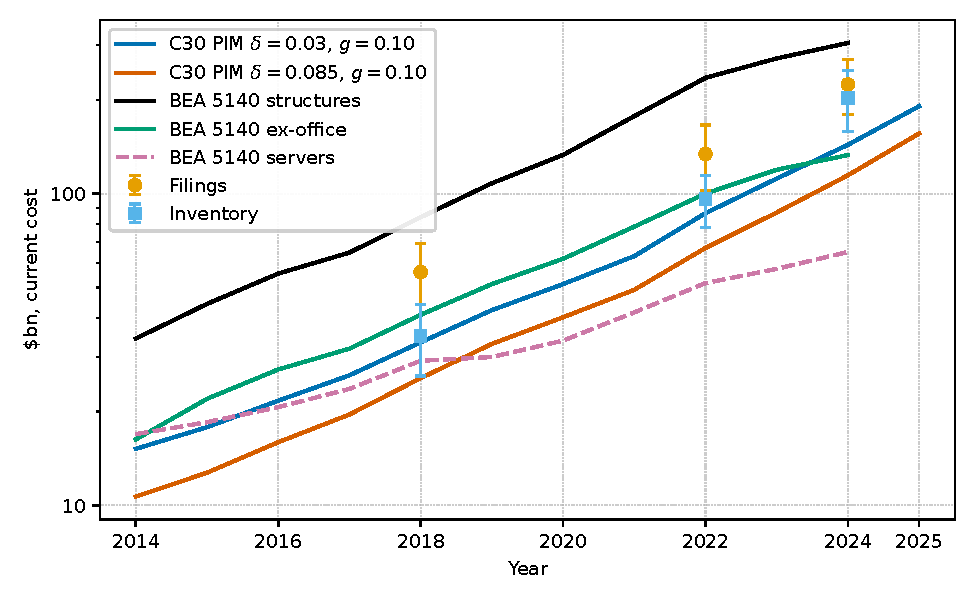
\includegraphics[width=\textwidth]{figures/dc_stock_sources.pdf}
\caption{US stock of data-center facilities by source, current cost, log scale. Lines: C30 cumulation at two depreciation rates; BEA industry 514 structures, total and excluding office; BEA industry 514 server equipment (dashed). Markers with ranges: filings (listed REITs plus hyperscalers plus private operators priced) and inventory estimates. Script: \texttt{data\_construction/dc\_stock\_sources.py}.}
\label{fig:sources}
\end{figure}

Four readings follow.

First, for 2018 the construction cumulation sits at the bottom of every other range. The listed colocation REITs alone hold \$23bn, which under the C30 stock of \$33bn leaves \$10bn for Google, Microsoft, Meta and AWS combined; the hyperscaler filings range starts at \$19bn. Filings with private operators, the inventory route and the fixed-asset total after an office deduction overlap at \$45--70bn. A central value of \$50bn is consistent with all three and with the construction cumulation under a low pre-sample growth rate ($g=0.05$ gives \$42bn).

Second, the fixed-asset total reconciles with filings once one asks who is in industry 514. If Alphabet, Meta, AWS and Microsoft all report their data centers in 514, as the establishment rule implies, then the industry's 2024 structures net of Alphabet's and Meta's offices (\$267--278bn) should equal the four companies' US data-center buildings (\$107--157bn) plus the colocation operators that are 518210 by activity (\$72--111bn) plus payment processors and other hosting establishments. The first two sum to \$179--268bn; the remainder, \$0--100bn, is the room for enterprise-serving hosting and for the low quality of the detail cells. If Microsoft is in software publishing and the REITs in real estate, the gap widens by about \$110--165bn and cannot be closed. The fixed-asset total is thus consistent with a broad reading of 514 and inconsistent with a narrow one.

Third, the sources move together over time. From 2018 to 2024 the construction stock rises 4.3 times, the fixed-asset total 3.6 times, filings with private operators about 4 times, and the inventory stock about 6 times. The inventory route grows fastest because it prices the whole stock at the 2024 cost per MW, 40\% above 2018, while book values in filings carry historical cost. The construction cumulation and the fixed-asset total, both at current cost, track each other closely in growth; the gap between them is a level gap that dates from before 2018.

Fourth, the disagreement between the two official series closes. Industry 514 structures investment was 2--4 times the C30 line in every year 2014--2022 and equal to it in 2024 (\$36.9bn against \$34.7bn). Either the Census line has caught up with hyperscale building as the data-center category matured, or the owner-industry accounts, which depend on company reporting in ACES, have begun to lag the boom. For nowcasting, the C30 line and the NIPA data-center structures series built on it are the only high-frequency official measures, and they now carry a smaller relative bias than in their early years.

\paragraph{Implications for calibration.} A facility stock built from construction spending is the right object and has the only usable flow series, but its level should be anchored to a year in which the pre-sample stock is a small share, or raised to match the filings and inventory ranges; for 2018 a factor of about 1.5 on the $g=0.10$ cumulation. The stock already contains power and cooling plant; a separate equipment stock for that plant should not be added, and its depreciation should be a blend near 0.085 rather than the office-building rate. JLL (2026) reports that 65\% of halls have a major power and cooling refresh by year 10 and almost all by year 15, which is the 10\% plant rate. Van Nieuwerburgh (2026) assigns a single 20-year life to building \emph{and} cooling (an annuity at a 10\% required return, not geometric $\delta$); that is the slower robustness case already computed, not the baseline. BEA industry 514 structures bound the stock from above and its server stock (\$29bn in 2018, \$65bn in 2024) is the natural companion series for the IT capital of the same establishments, with the same caveat that it covers all of 514. The type split within 514 changed materially between vintages and should not carry weight.

\section{Open items}

Two gaps remain. First, whether BEA places data centers under office structures since the 2025 update and which companies report in industry 514; a query to BEA's fixed-asset staff is pending. Second, operator-level capacity for the private colocation developers (full Structure Research tables, datacenterHawk), which would turn the residual-megawatt pricing into a count. The pre-2024 owned-megawatt series is no longer missing: JLL's mid-2026 report publishes 2017--26 inventory including owner-occupied halls. Whether those megawatts are facility power or IT load is still open (Van Nieuwerburgh's Cleanview caveat).

\appendix
\section{Hyperscaler inputs}
\label{app:hyp}

Table~\ref{tab:hyp} lists the inputs behind the hyperscaler rows of Table~\ref{tab:filings}. US data-center buildings, net $=$ gross buildings $\times$ net-to-gross $\times$ data-center share $\times$ US share, with net-to-gross 0.70--0.82 throughout.

\begin{table}[ht]
\centering
\begin{threeparttable}
\caption{Hyperscaler buildings and assumed data-center shares}
\label{tab:hyp}
\footnotesize
\begin{tabular}{llrccp{6.2cm}}
\toprule
Company & FY & Gross bldgs & DC share & US share & Basis for the data-center share \\
\midrule
Alphabet & 2018 & 30.2 & 0.40--0.55 & 0.75--0.79 & Land and buildings line ``includes offices, data centers''; HQ 11.2m sq ft is offices \\
 & 2022 & 66.9 & 0.45--0.60 & 0.72--0.76 & Same line; no split disclosed \\
 & 2024 & 55.8 & 1.00 & 0.74--0.77 & 40\% of technical infrastructure (\$139.6bn) is data-center land and buildings (2025 10-K) \\
Meta & 2018 & 7.4 & 0.75--0.90 & 0.75--0.78 & Offices mostly leased (7m sq ft); construction in progress ``mostly data centers'' \\
 & 2022 & 27.7 & 0.75--0.90 & 0.82--0.85 & Same; office consolidation under way \\
 & 2024 & 47.1 & 0.80--0.92 & 0.85--0.87 & Construction in progress no longer lists offices \\
Microsoft & 2018 & 20.6 & 0.65--0.85 & 0.73--0.76 & 10m sq ft owned King County offices of 24m owned total \\
 & 2022 & 55.0 & 0.70--0.88 & 0.74--0.77 & \$8.5bn committed construction ``primarily datacenters'' \\
 & 2024 & 93.9 & 0.75--0.90 & 0.74--0.76 & \$35.4bn committed ``primarily datacenters'' \\
Amazon & 2018 & 31.7 & 0.20--0.40 & 0.71--0.75 & AWS owned floor space 39\% of Amazon owned; AWS property \$18.9bn net \\
 & 2022 & 91.7 & 0.25--0.42 & 0.70--0.73 & AWS 35\% of owned floor space; AWS property \$60.3bn net \\
 & 2024 & 123.0 & 0.30--0.50 & 0.72--0.75 & AWS 36\%; AWS property \$110.7bn net; 60/40 split gives 47\% \\
Oracle & 2018 & 3.9 & 0.10--0.30 & 0.66--0.70 & Own and colocation data centers \\
 & 2022 & 4.7 & 0.05--0.20 & 0.62--0.66 & ``Substantially all'' data centers leased through colocation \\
 & 2024 & 6.5 & 0.05--0.20 & 0.75--0.78 & Same \\
\bottomrule
\end{tabular}
\begin{tablenotes}\footnotesize
\item Gross buildings in \bn\ from the PP\&E note (Alphabet 2018 and 2022 is ``land and buildings''). US share from property or long-lived assets by geography; for Microsoft from owned floor space, because its long-lived assets include Irish and Luxembourg intangibles. Microsoft fiscal years end in June.
\end{tablenotes}
\end{threeparttable}
\end{table}

\section*{Sources}

\begin{itemize}
  \item Census Bureau, Value of Construction Put in Place, private seasonally adjusted series, data-center line 2014--2026; definitions and methodology pages.
  \item BEA, Detailed Data for Fixed Assets and Consumer Durable Goods by industry (net stocks, investment, depreciation, implied rates), August 2019 and September 2025 releases; \emph{BEA depreciation rates}; \emph{Fixed Assets and Consumer Durable Goods in the United States, 1925--97}, methodology; Survey of Current Business, September 2011; BEA working paper 2025-8.
  \item Census Bureau, 2022 NAICS Manual, introduction (auxiliary establishments) and 518210; ACES form ACE-1 instructions, item 6A.
  \item SEC EDGAR XBRL company facts and 10-K filings for Equinix, Digital Realty, CyrusOne, QTS, CoreSite, Iron Mountain, Alphabet, Microsoft, Amazon, Meta, Oracle.
  \item CBRE North America Data Center Trends, H2 2018, H2 2021, H2 2022, H2 2024; Structure Research US data-centre markets 2024 and 2025 (executive summaries) and hyperscale self-build 2023; JLL North America Data Center Report, mid-year 2026 (file label YE 2026) and mid-year / year-end 2025; Synergy Research hyperscale counts 2018, 2023, 2024.
  \item Turner \& Townsend Data Centre Cost Index 2018, 2020, 2022, 2024, 2025; Uptime Institute provisioning cost notes; JLL 2026 Global Data Center Outlook (January 2026).
  \item Van Nieuwerburgh, S.\ (2026), ``Financing the AI Buildout,'' Brookings Papers on Economic Activity, draft 4 September 2026. Cleanview project file (July 2026) and the 200~MW campus bill (Appendix A).
  \item Shehabi et al., LBNL United States Data Center Energy Usage Reports, 2016 and 2024, and 2025 update.
\end{itemize}

\end{document}
